\documentclass[11pt]{standalone}
\usepackage{pgf, tikz}
\usetikzlibrary{arrows, automata}

\begin{document}
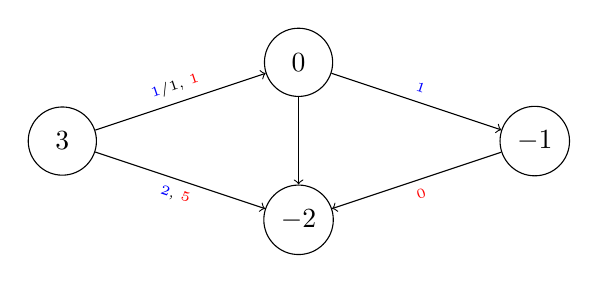
\begin{tikzpicture} [align=center]
\path (3, 0) node[circle, draw, text width=0.5cm] (v0) {$3$}
      (6, 1) node[circle, draw, text width=0.5cm] (v1) {$0$}
      (6, -1) node[circle, draw, text width=0.5cm] (v2) {$-2$}
      (9, 0) node[circle, draw, text width=0.5cm] (v3) {$-1$};
      
\draw[->] (v0) to node [sloped, anchor=center, above] {\tiny \textcolor{blue}{1}/1, \textcolor{red}{1}} (v1);
\draw[->] (v0) to node [sloped, anchor=center, below] {\tiny \textcolor{blue}{2}, \textcolor{red}{5}} (v2);
\draw[->] (v1) to node [sloped, anchor=center, above, blue] {\tiny 1} (v3);
\draw[<-] (v2) to node [sloped, anchor=center, below, red] {\tiny 0} (v3);
\draw[->] (v1) to (v2);

\end{tikzpicture}
\end{document}